% -*- mode:LaTeX; mode:visual-line; mode:flyspell; fill-column:75 -*-
\section{Experiments and Results}
\label{sec:results}

We now present proof-of-concept experiments on a robot reaching task.
These early results serve as an initial demonstration of our ability to learn the correct behavior from user demonstrations and apply those when the user provides natural language command during task execution.

The robot is tasked with reaching a goal, and as the initial Dynamical System is a linear dynamics model with a stable attractor at the goal position this results in straight-line trajectories towards the goal.
While this initial behavior correctly specifies the task (the \emph{what}), changes in the environment (such as the addition of a basket) may result in the robot incorrectly performing the task, as shown in \Cref{figExperimentSetup}.
Note that in our experiments the robot has no sensors to detect obstacles.
The training phase consisted of a single demonstration with the user back-driving the robot under the original dynamics with the utterance ``go up''.

During the experiment, the user helps the robot to complete the task correctly by reshaping the Dynamical System using the learned correction (invoked using the same natural language utterance).
In this work we used text-based input with no delay; using a speech-to-text engine would be straightforward but would introduce additional delays, handling those remains future work.
In this scenario the robot is able to complete the task without hitting the box with the modified DS, and can generalize to different starting positions.
Additionally, using the same learned correction the user could modify the dynamics on a different task (reaching inside a box in another location) with the same utterance.

\begin{figure}[t]
  \centering
  \begin{tikzpicture}
    \draw (0, 0)
    node[name=image, anchor=south west, inner sep=0pt, outer sep=0pt]{
      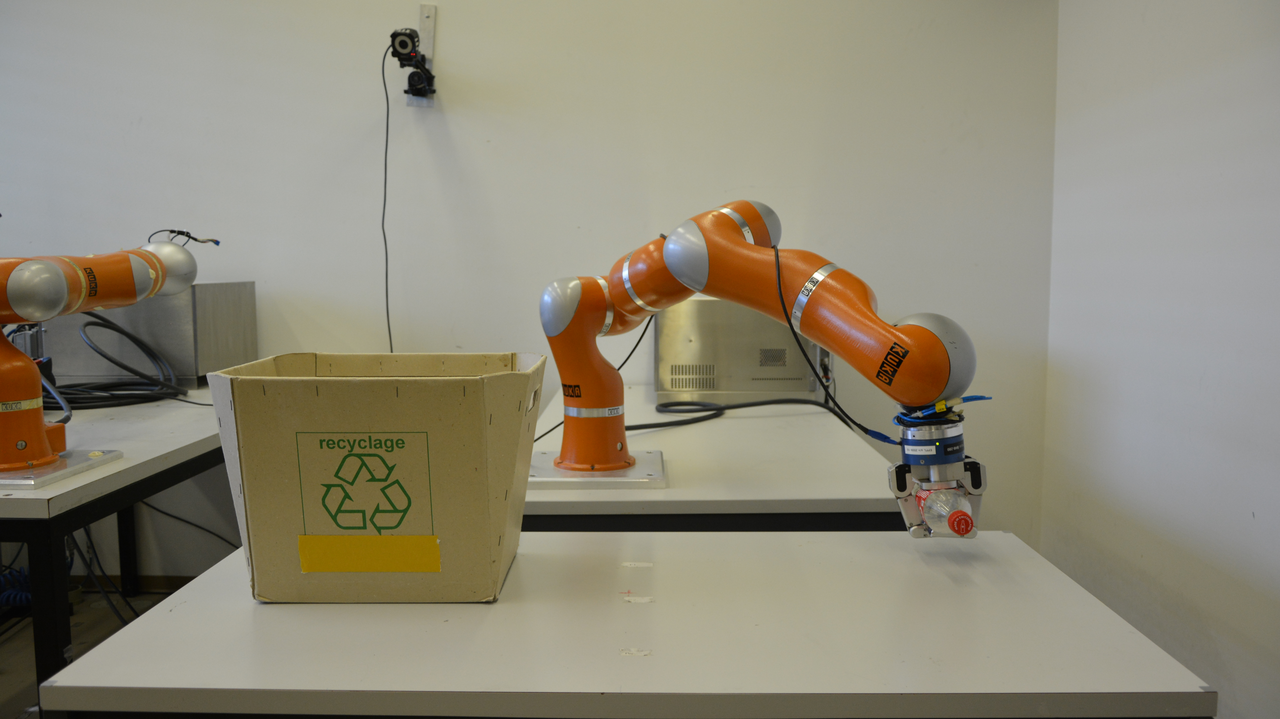
\includegraphics[
        % trim = left bottom right top
        trim = 18mm 5mm 20mm 15mm, clip,
        width = 0.4\textwidth
      ]{figs/setup-start.png}
    };
    \begin{scope}[x={(image.south east)},y={(image.north west)}]

      %% Grid
      %% \draw[help lines,xstep=.1,ystep=.1] (0,0) grid (1,1);
      %% \foreach \x in {0,1,...,9} { \node [anchor=north] at (\x/10,0) {0.\x}; }
      %% \foreach \y in {0,1,...,9} { \node [anchor=east] at (0,\y/10) {0.\y}; }

      \node[] (goal) at (0.2, 0.4) {};
      % List all the starting positions here (first is the actual hand).
      \foreach \x/\y in {0.85/0.3, 0/0, 0.6/0.1, 0.2/0.9, 0.4/0.9, 0.9/0.8} {
        \node[] (start) at (\x, \y){};
        \draw[->, blue, ultra thick, shorten >= 5pt] (start) -- (goal);
      }

    \end{scope}
  \end{tikzpicture}
  \caption{
    From the start position shown, the robot must place the bottle into the basket.
    However, the initial Dynamical System is unaware of the geometry of the basket, and the original trajectories are straight lines (shown in blue).
    Using the language description ``go up,'' the robot is able to infer a modification to the DS in order to execute the task correctly.
  }
  \label{figExperimentSetup}
\end{figure}
